Modeling the transition between different nuclear fuel cycles provides 
information on the quantity and timing of various materials to meet 
specific objectives, such as providing fuel for reactors to meet a 
prescribed energy demand. 
This work models potential transitions from the 
current fleet of \glspl{LWR} in the US to advanced reactors to quantify the 
resources required to support the transition. I used 
\Cyclus \cite{huff_fundamental_2016} to simulate all of the transitions 
in this 
work, with each of the fuel cycle facilities (including reactors) defined 
through the \Cycamore archetype library \cite{carlsen_cycamore_2014}. Each 
simulation models current 
\glspl{LWR} starting in 1965 and models all reactors out to 2090 with a timestep 
of one month. The \gls{IAEA} \gls{PRIS} database \cite{noauthor_power_1989} 
provided the start and select end dates for \glspl{LWR}. The \gls{PRIS} database 
only contains end dates for reactors shut down before the publication of the 
database each year. Reactors still operating in December 2020  
lack an end date in the \gls{PRIS} database and are assumed to operate 
until 
their current operating license expiration date, obtained from 
\cite{nuclear_energy_institute_us_2021}. This work considers only 
reactors in the \gls{PRIS} database with a power level above 400 MWe 
to avoid including prototype and research reactors present in the database. 
Approximate masses for fuel used in the cores of the \glspl{LWR} were obtained 
from \cite{todreas_nuclear_2012} and \cite{cacuci_handbook_2010}. 

This work models the transition to advanced reactors assuming a 
once-through fuel cycle. The scenarios are defined based 
on the energy demand 
of the scenario (either no growth or 1\% annual growth in demand) and by the 
advanced reactors deployed in the scenario. The transition from \glspl{LWR} 
to advanced reactors begins in January 2025, so the energy generated by 
\glspl{LWR} in 2025 is the basis for the energy demand in each scenario.  
Many of the 
current plans for \gls{HALEU}-fueled reactors do not have these reactors 
deployed until the late 2020s \cite{nichol_current_2021} through \gls{ARDP} 
and other programs. I selected 2025 as the transition 
start time for this work because it will provide a bounding case for 
an aggressive deployment of these reactors. 

This work compares the fuel cycle scenarios on various metrics: 
the energy produced, the number of reactors deployed, the 
uranium usage (both enriched uranium required for fuel and feed uranium 
to produce enriched uranium), 
the \gls{SWU} capacity required to produce the enriched uranium, and the 
amount of waste produced. Comparisons of the energy generated will ensure 
that demand is fully met and identify any disadvantages in deploying each 
reactor type or flaws in the methodology. One would expect that the
number of reactors built to meet the energy demand will be a major 
factor in deciding which reactors to deploy, which led to the 
consideration of this component of the transitions. The uranium usage 
will provide insight into the facility throughput and raw materials 
required to support the 
transition. The \gls{SWU} capacity informs on the enrichment facility 
capacity required to support the transition. Comparisons of the transition 
\gls{SWU} capacity to current capacities will inform on if new facilities 
are required. Finally, the waste produced, specifically the \gls{SNF} 
discharged from the reactors, informs on potential repository capacities 
required for final disposal of the waste. The natural 
uranium usage and waste production are two of the metrics used in the 
\acrfull{ES} 
\cite{wigeland_nuclear_2014}, and the mass of enriched uranium was the 
primary result of the work by Dixon et al. \cite{dixon_estimated_2022}, 
which contributed to the development of this list of material 
requirements to compare.

\section{Advanced reactor modeling} \label{sec:reactor_methods}
This work considers three advanced reactors: the \gls{USNC} \gls{MMR}, 
\cite{noauthor_usnc_2021,mitchell_usnc_2020}, the X-energy Xe-100 
\cite{mulder_overview_2021}, and 
the NuScale VOYGR reactor
\cite{nuscale_chapter_2020-1,reyes_nuscale_2021,reyes_correction_2022}. The 
\gls{USNC} \gls{MMR}
and X-energy Xe-100 reactors require \gls{HALEU}, but the NuScale VOYGR 
requires \gls{LEU} with a similar enrichment level to current \gls{LWR} fuel 
(Table \ref{tab:reactor_summary}). This work includes the NuScale VOYGR, 
despite not requiring \gls{HALEU} fuel, 
because the \gls{NRC} granted it design approval \cite{world_nuclear_news_nuscale_2021} 
and it is very likely to be 
deployed along-side \gls{HALEU}-fueled reactors. Including the  
VOYGR reactor in the transition scenarios provides insight into how the 
deployment of \gls{HALEU}-fueled and non-\gls{HALEU}-fueled advanced 
reactors in tandem 
affects the material requirements of the transition. However, because the 
VOYGR reactor does not require 
\gls{HALEU}, this work does not consider the transition from \glspl{LWR} 
to only the VOYGR.

\begin{table}[ht]
    \centering
    \caption{Advanced reactor design specifications.}
    \label{tab:reactor_summary}
    \renewcommand{\arraystretch}{1.5}
    \begin{tabular}{p{3.5cm}p{3cm}p{3cm}p{3cm}}
        \hline
        Design Criteria & \gls{USNC} \gls{MMR} \cite{noauthor_usnc_2021} & 
        X-energy Xe-100 \cite{mulder_overview_2021} & NuScale VOYGR 
        \cite{nuscale_chapter_2020-1,reyes_nuscale_2021,reyes_correction_2022}\\
        \hline
        Reactor type & Modular HTGR & Modular HTGR & SMR\\
        Power Output (MWth) & 15 & 200  & 250 \\
        Capacity Factor & 100\% & 95\% & 95\% \\
        Enrichment (\% $^{235}U$) & 19.75 & 15.5 & <4.95 \\
        Cycle Length (yrs) & 20 & online refuel & 1.5\\
        Number of cycles & 1 & 6 & 3\\
        Fuel form & UO$_2$ \gls{FCM} compacts & UCO \gls{TRISO} pebbles & UO$_2$ pellets\\
        Discharge fuel burnup (GWd/MTU) & 82 & 168  & 45 \\
        Reactor Lifetime (yrs)& 20 & 60 & 60 \\
        \hline
    \end{tabular}
\end{table}

Defining a reactor with the \Cycamore \texttt{Reactor} archetype, 
requires knowing the refueling scheme and the fuel composition for 
the reactor. The refueling scheme includes 
the cycle time, the refueling time, and the mass of fuel put into the reactor 
at each refueling. The parameters for the reactors (Table \ref{tab:reactor_summary})
are meant to closely match the design information about each reactor that 
is available through open-source information. The fuel mass required by 
each reactor type was calculated based on the reactor thermal power, 
cycle length, and burnup:

\begin{equation}
    \text{mass [kg] = }\frac{\text{Power [MWth]}* \text{cycle 
    length [d]} * \text{number of cycles}}{\text{burnup [MWd/kg]}}
    \label{eq:fuel_mass}
\end{equation}

\noindent Eq. \ref{eq:fuel_mass} calculates the mass of uranium required 
in the core. To calculate the total mass of the fuel (including the carbon 
and/or oxygen in the fuel) this value was divided by the mass fraction of 
uranium in the fuel form for the reactor. Any non-uranium components 
of the fuel, such as silicon-carbide in \gls{TRISO} particles, were 
not considered in the mass. This methodology assumes that the 
uranium and uranium-containing fuel components would be the limiting 
factor in the fuel cycle and other fuel components would be available as 
needed. 

The \gls{MMR} does not undergo refueling, the initial core
burns for the entire lifetime of the reactor \cite{mitchell_usnc_2020}. 
Therefore, the \gls{MMR}
does not include any down time for refueling and has a cycle length that 
matches the reactor lifetime. Additionally, the refueling mass for the
\gls{MMR} is zero. 

The Xe-100 undergoes online refueling operations, with each 
\gls{TRISO} pebble passing 
through the reactor six times before discharge \cite{mulder_overview_2021}. 
Every six months about 1/7th 
of the pebbles in the core are expected to be discharged. The Xe-100 
refueling is modeled as a refueling time of zero months and a 
replacement of 1/7th of the core mass every 
6 months.  

The VOYGR contains 37 fuel assemblies, with three different enrichment 
levels \cite{nuscale_chapter_2020-1}. Each refueling replaces 13 fuel 
assemblies, with the middle assembly replaced at every refueling. 
Therefore 13/37th of the core mass is replaced at each refueling. 
The fuel enrichment used is an average of the assembly enrichments 
presented in \cite{nuscale_chapter_2020-1}. NuScale reports that a refueling 
outage for the VOYGR will take ten days \cite{nuscale_nuscale_2022}. However 
the smallest timestep modeled in this work is one month, therefore this 
work models a VOYGR 
refueling outage is modeled as one month. 

Fresh fuel 
recipes for the advanced reactors are based on the 
defined fuel form for each reactor using the appropriate uranium isotope 
ratio for enrichment. Both the \gls{MMR} and VOYGR are intended to be built 
in sets (2 \gls{MMR} per site \cite{noauthor_usnc_2021} and up to 12 VOYGR 
units per site \cite{reyes_nuscale_2021}), but in this study every reactor 
design is treated 
on a single unit basis. Therefore, the number of reactors built in each 
of the transitions does not represent the number of unique sites required 
to build the reactors. All cores modeled are assumed to be equilibrium cores, 
this work does not consider start-up cores or the transition to equilibrium. 

To properly account for the capacity factor of each reactor, the power output 
(in MWe) of each reactor was multiplied by the capacity factor and explicit 
modeling of outages was removed. This methodology was applied to the 
advanced reactors and the current fleet of \glspl{LWR}, which were assumed 
to operate with a 92.66\% capacity factor based on the last five years of 
fleet-averaged capacity factors \cite{us_energy_information_administration_electric_2022}. 
By removing 
explicit modeling of outages, the outages do not artificially affect 
the capacity factors. The operating cycle of the \glspl{LWR} and VOYGRs 
was extended by 1 time step, to ensure that these facilities received fuel 
on the same schedule as if the outages were explicitly modeled. 

\section{Once-through fuel cycle} \label{sec:once-through-methods}
Figure \ref{fig:once-through_fuel_cycle} shows the flow of material through 
the modeled once-through fuel cycles. The once-through fuel cycle models 
material from the mine to final disposal in a repository (the 
``HLW Sink'' in Figure \ref{fig:once-through_fuel_cycle}). The 
``Advanced Reactor'' node in Figure 
\ref{fig:once-through_fuel_cycle} represents any subset of the advanced 
reactors (Xe-100s, \glspl{MMR}, and VOYGRs) included 
in the scenario. This model assumes that all enriched uranium is produced 
by enriching natural uranium; downblending \gls{HEU} is not considered. 
This fuel cycle is a simplified version of the modeled fuel cycle in 
\cite{bachmann_enrichment_2021}, removing steps in the fuel cycle that 
do not affect the reported results. Removing some of the steps simplified 
the models from a user standpoint and reduced the size of the \Cyclus 
output file, facilitating data analysis. The transition from the 
\glspl{LWR} to the advanced reactors begins in 2025. Each of the non-reactor 
facilities have an unlimited capacity to produce or process materials,
to prevent material unavailability from influencing the results. 
This methodology has previously been applied to transition analysis 
\cite{djokic_application_2015}.

\begin{figure}
    \centering
    \begin{tikzpicture}[node distance=1.5cm]
        \node (mine) [facility] {Uranium Mine};
        \node (enrichment) [facility, below of=mine]{Enrichment};
        \node (reactor) [facility, below of=enrichment]{Reactor};
        \node (adv_reactor) [transition, right of=reactor, xshift=3cm]{Advanced Reactor};
        \node (wetstorage) [facility, below of=reactor]{Cooling Pool};
        %\node (drystorage) [facility, below of=wetstorage]{Dry Storage};
        \node (cooling) [transition, below of=adv_reactor]{Cooling Pool};
        \node (sinkhlw) [facility, below of=wetstorage, xshift=2.5cm]{HLW Sink};
        \node (sinkllw) [facility, left of=enrichment, xshift=-3cm]{LLW Sink};

        \draw [arrow] (mine) -- node[anchor=east]{Natural U} (enrichment);  
        \draw [arrow] (enrichment) -- node[anchor=south]{Tails}(sinkllw);
        \draw [arrow] (enrichment) -- node[anchor=east]{Fresh UOX}(reactor);
        \draw [arrow] (enrichment) -| node[anchor=west]{Fresh HALEU and LEU}(adv_reactor);
        \draw [arrow] (reactor) -- node[anchor=east]{Spent UOX}(wetstorage);
        \draw [arrow] (wetstorage) |- node[anchor=east]{Cool Spent UOX}(sinkhlw);
        %\draw [arrow] (drystorage) |- node[anchor=east]{Casked Spent UOX}(sinkhlw);
        \draw [arrow] (adv_reactor) -- node[anchor=west]{Spent Fuel}(cooling);
        \draw [arrow] (cooling) |- node[anchor=west]{Cooled Spent HALEU and LEU}(sinkhlw);`'

        \end{tikzpicture}
    \caption{Fuel cycle facilities and material flow between facilities in the 
    once-through fuel cycles modeled. Facilities in 
    blue are used in all once-through scenarios, the facilities in red are added in
    at the transition start time in the transition scenarios.}
    \label{fig:once-through_fuel_cycle}
\end{figure}

The once-through scenarios model the current fleet of \glspl{LWR} in the 
US and the transition to multiple 
combinations of the advanced reactors and different energy demand scenarios, 
summarized in Table \ref{tab:scenarios_once-through}. Scenario 1 models
the \gls{LWR} fleet without the transition to any advanced reactor to 
provide 
a comparison with historic needs for a fuel cycle 
based on enrichments to less than 5\% $^{235}$U. The energy demands are 
based on the energy supplied by the \glspl{LWR} in 2025 (the start of 
the transition). A no growth energy demand applies a constant demand for 
the energy produced by \glspl{LWR} in 2025, and a 1\% growth demand applies 
an exponential growth demand starting at the energy produced by 
\glspl{LWR} in 2025. A 1\% annual growth in 
demand (Scenarios 8-13) is less than what Dixon et al. \cite{dixon_estimated_2022} 
modeled
(1.2\%-2\%) but more than the average growth between 2020-2050 in the 
reference case of the 2022 \gls{EIA} Annual Energy Outlook 
\cite{us_energy_information_administration_annual_2022} (0.82\%), and 
provides a middle-ground estimate on material requirements for a growing 
energy demand. 

\begin{table}[ht]
    \centering
    \caption{Summary of the once-through fuel cycle transition scenarios.}
    \label{tab:scenarios_once-through}
    \begin{tabular}{l l l}
            \hline
            Scenario number & Reactors present & Energy growth model\\\hline
            1 & \glspl{LWR} & N/A \\
            2 & \glspl{LWR} and \gls{MMR} & No growth \\
            3 & \glspl{LWR} and Xe-100 & No growth \\
            4 & \glspl{LWR}, Xe-100, and \gls{MMR}& No growth\\
            5 & \glspl{LWR}, \gls{MMR}, and VOYGR & No growth\\
            6 & \glspl{LWR}, Xe-100, and VOYGR & No growth\\
            7 & \glspl{LWR}, Xe-100, \gls{MMR}, and VOYGR & No growth\\
            8 & \glspl{LWR} and \gls{MMR}& 1\% growth \\
            9 & \glspl{LWR} and Xe-100 & 1\% growth\\
            10 & \glspl{LWR}, Xe-100, and \gls{MMR}& 1\% growth\\
            11 & \glspl{LWR}, \gls{MMR}, and VOYGR & 1\% growth\\
            12 & \glspl{LWR}, Xe-100, and VOYGR & 1\% growth\\
            13 & \glspl{LWR}, Xe-100, \gls{MMR}, and VOYGR & 1\% growth\\
            \hline
    \end{tabular}
\end{table}

Recipes define the composition of each material in the simulation. 
Recipes for \gls{LWR} fresh and spent fuel were found in work 
by Jacobson et al. \cite{jacobson_verifiable_2010}.
Section \ref{sec:reactor_methods} describes how I obtained recipes for 
fresh 
fuel of the advanced reactors. Other important recipes in the simulations include 
natural uranium (0.711\% weight fraction $^{235}$U) and enrichment tails 
(0.2\% weight fraction $^{235}$U).

The institutions in the simulations 
govern the deployment of reactors. A \Cycamore \texttt{DeployInst} 
institution \cite{huff_fundamental_2016} deploys and decommissions the 
\glspl{LWR} according to their start and end dates. A second \Cycamore 
\texttt{DeployInst} deploys and decommissions the advanced reactors, 
based on calculations, external to the \Cyclus simulations, of when 
new reactors must be deployed to meet the energy 
demand. All of the facilities and institutions in the simulation are in 
the same region, which represents that all facilities are in the same 
country. No  
tariffs are modeled on the commodity transactions.

The advanced reactor deployment scheme
preferentially deploys the advanced reactor with the largest power 
output in the scenario (e.g., Xe-100s in Scenario 7) until their 
deployment would create an oversupply of power. Then the next reactor 
is deployed until an oversupply of power would be created. Finally, the 
reactor 
with the smallest power output in the scenario (e.g., \glspl{MMR} in 
Scenario 7) are deployed until their deployment creates a small oversupply 
of power (i.e., the number of reactors needed is rounded up). The demand 
to be met by deploying new reactors is the difference between the energy 
produced and the energy demand at each time step. 
Figure \ref{fig:AR_deployment} illustrates how the advanced reactors 
would be deployed in Scenario 7 to meet a demand of 480 MWe. For this 
example, 5 Xe-100s, 1 VOYGR, and 1 \gls{MMR} are deployed, producing a 
total of 482 MWe. This deployment 
strategy aims to minimize the number of reactors deployed,  
minimize power oversupply, and mimic a realistic deployment strategy.

\begin{figure}[ht]
    \centering
    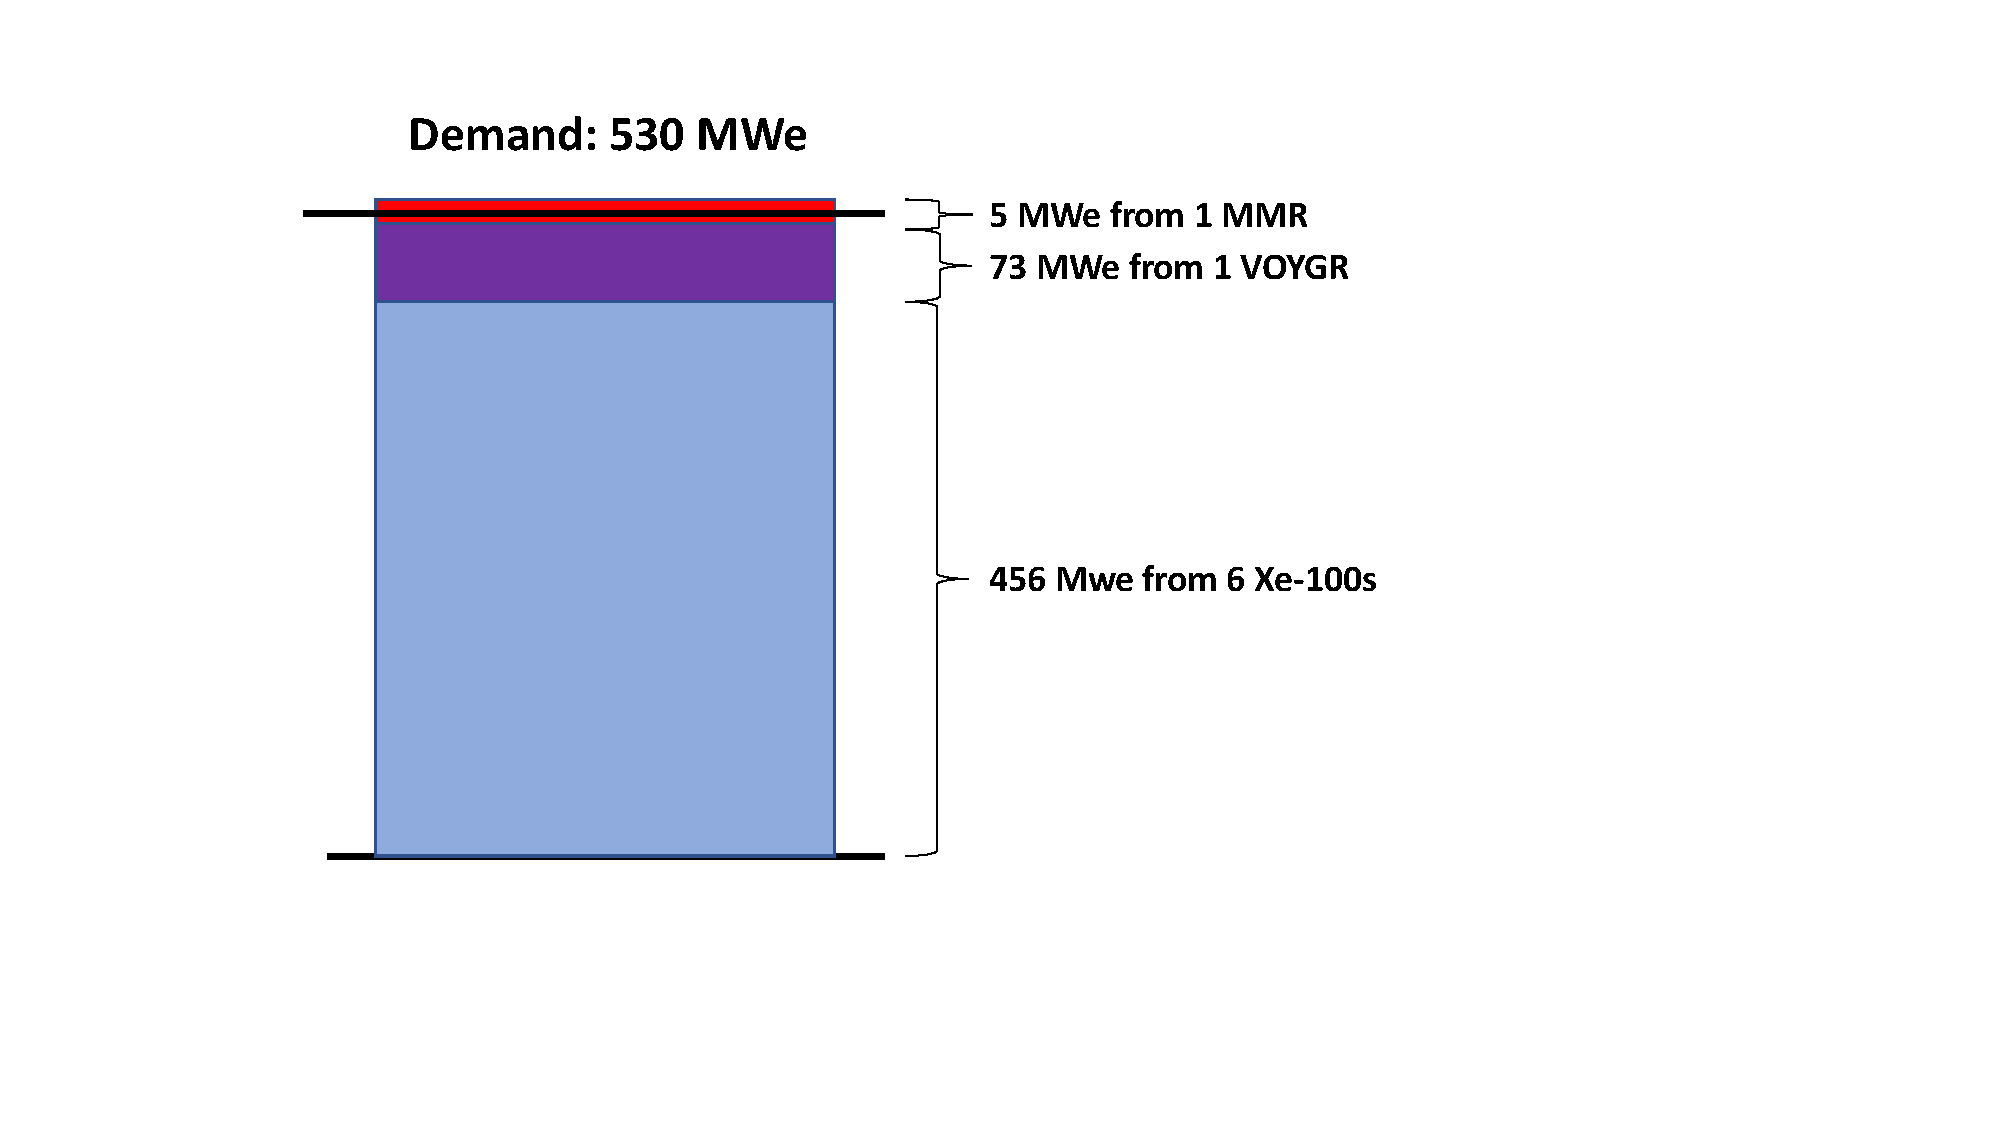
\includegraphics[scale=0.6, trim=50 100 60 0,clip]{Deployment_Scheme.pdf}
    \caption{Example of how advanced reactors are deployed in Scenario 7 
    to meet a demand of 480 MWe.}
    \label{fig:AR_deployment}
\end{figure}

This deployment scheme for advanced reactors applies when there is an 
unmet demand in energy from the decommissioning of \gls{LWR} or 
when the demand increases (such as in the 1\% growth scenarios). When 
there is unmet demand from the decommissioning of advanced reactors, the 
advanced reactors are redeployed on almost a one-to-one basis. A slightly
smaller number of advanced reactors may be redeployed if there is an 
oversupply of power greater than the power output of the reactor to be 
redeployed. 

\section{Recycling fuel cycle}
Transition scenarios with a closed fuel cycle were created
to investigate how this type of \gls{NFC} affects the material requirements 
and how the recycling scheme impacts them. 
The scenarios investigated in this analysis vary by the 
energy demand of the scenario and the recycling scheme (Table 
\ref{tab:scenarios_recycle}). Energy demands vary 
between a no growth and a 1\% growth model, the same as the variation in this 
parameter in the once-through fuel cycle models. Variations in the recycling 
scheme include either a limited or a continuous recycle. Limited recycle 
scenarios assume that \gls{SNF} is recycled once and disposed of after a 
second pass through the reactor. Continuous recycling assumes that all 
\gls{SNF} is recycled an unlimited number of times until all fissile 
material has been used. Both recycling schemes were considered in the 
\acrfull{ES} \cite{wigeland_nuclear_2014}, which is why they are both 
considered in this work. Another distinction between some of the 
scenarios is if \gls{TRISO} fuel is recycled. \gls{TRISO} fuel is 
expensive and difficult to recycle \textbf{find citation}, and 
therefore by modeling scenarios that do and do not recycle 
\gls{TRISO} we can model realistic scenarios in which \gls{TRISO} 
is recycled and more academic scenarios in which all spent fuel is 
recycled. 

\begin{table}[ht]
    \centering
    \caption{Summary of the recycle fuel cycle transition scenarios.}
    \label{tab:scenarios_recycle}
    \begin{tabular}{l l l l}
            \hline
            Scenario number & Energy growth model & Recycle scheme & TRISO recycled?\\
            \hline
            14 & No growth & Limited & Yes\\
            15 & No growth & Limited & No\\
            16 & No growth & Continuous & ??? \\
            17 & 1\% growth & Limited & Yes\\
            18 & 1\% growth & Limited & No\\
            19 & 1\% growth & Continuous & ??? \\
            \hline
    \end{tabular}
\end{table}

All of the scenarios with recycling model the transition from the 
current fleet of \glspl{LWR} to the X-energy Xe-100, \gls{USNC} \gls{MMR}, 
and the NuScale VOYGR, the same as in scenarios 7 and 13. Therefore, 
the advanced reactor deployment schedules for these two scenarios are applied 
to the recycling scenarios for the appropriate energy growth model. 
This combination 
of reactors is considered for this step of the work, and not all of the 
combinations considered for the once-through scenarios, to limit the scope 
of the work while providing some amount of comparison between the 
once-through and recycle transition scenarios. Because these scenarios 
use the same advanced reactor deployment schedule, the number of 
advanced reactors and the energy supplied are not examined in the 
results because they will be the same for each of these scenarios. Instead, 
the results of these scenarios will focus on the material requirements. 

\subsection{Limited recycle scenarios}
Figure \ref{fig:limited_recycle_flow} shows the fuel cycle and material flows 
for the scenarios with limited recycling (Scenarios 14, 15, 17, and 18). 
In scenarios 15 and 18 only the spent fuel from the \glspl{LWR} and 
VOYGRs is sent to the reprocessing facility, but in scenarios 14 and 17, 
all spent fuel from the advanced reactors and \glspl{LWR} is sent to the 
reprocessing facility. \gls{MOX} fuel is not sent to the \gls{MMR} in this 
material flow scheme because the \gls{MMR} does not undergo refueling, 
and therefore would not receive \gls{MOX} fuel. 

\begin{figure}
    \centering
    \begin{tikzpicture}[node distance=1.5cm]
        \node (mine) [facility, text width=1cm] {Uranium Mine};
        \node (enrichment) [facility, below of=mine]{Enrichment};
        \node (reactor) [facility, below of=enrichment]{LWR};
        \node (mmr) [transition, right of=reactor, xshift=1.5cm]{MMR};
        \node (xe100) [transition, right of=mmr, xshift=1.5cm]{Xe-100};
        \node (voygr) [transition, right of=xe100, xshift=1.5cm]{VOYGR};
        \node (wetstorage) [facility, below of=reactor, text width=1cm]{Cooling Pool};
        \node (drystorage) [facility, below of=wetstorage, text width=1.5cm]{Dry Storage};
        \node (cooling) [transition, below of=mmr, xshift=1.5cm, text width=1cm]{Cooling Pool};
        \node (sinkhlw) [facility, below of=drystorage, xshift=2.5cm, yshift=-1cm]{Repository};
        \node (sinkllw) [facility, left of=enrichment, xshift=-1.5cm, text width=1cm]{Tails Sink};
        \node (separation) [transition, below of=cooling, yshift=-1cm]{Separations};
        \node (mox_fab) [transition, below of=voygr,xshift=2cm, text width=1cm]{MOX Fuel Fab};
        \node (mox_cooling) [transition, below of=xe100, xshift=1.5cm, yshift=-1.5cm]{MOX Cooling};
        
        \draw [arrow] (mine) -- node[anchor=west]{Natural uranium} (enrichment);
        \draw [arrow] (enrichment) -- node[anchor=east]{Fresh UOX}(reactor);
        \draw [arrow] (enrichment) -- node[anchor=south]{Tails}(sinkllw);
        \draw [arrow] (enrichment) -| (mmr);
        \draw [arrow] (enrichment) -| node[anchor=south]{Fresh UOX}(xe100);
        \draw [arrow] (enrichment) -| (voygr);
        \draw [arrow] (reactor) -- node[anchor=east]{Spent UOX}(wetstorage);
        \draw [arrow] (wetstorage) -- node[anchor=east]{Cool Spent UOX}(drystorage);
        \draw [arrow] (drystorage) |- node[anchor=east]{Casked Spent UOX}(sinkhlw);
        \draw [arrow] (mmr) |- node[anchor=east]{Spent UOX}(cooling);
        \draw [arrow] (xe100) |- (cooling);
        \draw [arrow] (voygr) |- node[anchor=south]{Spent UOX}(cooling);
        \draw [arrow] (xe100) -| (mox_cooling);
        \draw [arrow] (voygr) -| node[anchor=south, text width=1cm, pos=0.25]{Spent MOX}(mox_cooling);
        \draw [arrow] (cooling) -- node[anchor=west, text width=1.5cm]{Cooled Spent UOX}(separation);
        \draw [arrow] (separation) -| node[anchor=south,text width=1.5cm, pos=0.4]{Separated fissile material}(mox_fab);
        \draw [arrow] (separation) -| node[anchor=south, text width=1.5cm]{Fission Products}(sinkhlw);
        \draw [arrow] (mine) -| node[anchor=south, pos=0.4]{Natural uranium} (mox_fab);
        \draw [arrow] (mox_cooling) |- node[anchor=south]{Cool Spent MOX}(sinkhlw);
        \draw [arrow] (mox_fab.east) - ++(5mm,0) |- node[anchor=south, pos=0.5, text width=1.5cm]{Fresh MOX}(voygr.east);
        %\draw [arrow] (mox_fab.east) -| ++(5mm,0) -| (xe100.north);
        \end{tikzpicture}
    \caption{Fuel cycle facilities and material flow between facilities for modeling the transition 
    to advanced reactors with a limited recycle fuel cycle. The separations facility
    is deployed in 2020, five years before the transition. Before 2020 a once-through 
    fuel cycle is used with the facilities in blue.}
    \label{fig:limited_recycle_flow}
\end{figure}

A separations facility is defined to be deployed 5 
years before the transition 
begins (i.e. in 2020), as this strategy is commonly used for modeling 
transitions with recycling \cite{passerini_systematic_2014,richards_application_2021}
to ensure that enough fuel can be separated and 
processed in time for use in advanced reactors. Although this is a 
non-physical time to begin recycling in the US, using this timeline ensures 
that there will be enough reprocessed fuel to fuel all of the advanced 
reactors. The deployment time of the separation facility will be adjusted 
to determine if a more physical deployment timeline is possible. Additionally, 
by using this timeline, specifically ensuring that advanced reactors 
are deployed at the same time as when they are deployed in the once-through 
transition to provide an even comparison between these fuel cycle options.

The separations facility separates out uranium and plutonium from the other 
materials in the fuel, emulating the COEX reprocessing method although the 
chemistry is not explicitly modeled. The separation efficiency is \textbf{find 
these numbers} for plutonium and uranium, respectively. The separated 
material from this facility is then sent to a \gls{MOX} fuel fabrication 
facility that produces \gls{MOX} with a pre-defined composition for each 
advanced reactor \textbf{found from literature, transport calculations, 
or plutonium equivalence}.
The separated plutonium is used as a fissile stream while the separated 
uranium and natural uranium from the mine are used as filler materials to 
produce the \gls{MOX}.

\subsection{Continuous recycle scenarios}
Figure \ref{fig:continuous_recycle_flow} shows the facilities and material 
flow for the continuous recycle fuel cycle. Continuous recycle 
requires a fast reactor, and all of the reactors considered in this 
work have a thermal neutron energy spectrum. Therefore, a fast reactor 
facility 
must be added into the transition. To accomplish this, two different 
transitions are included in these scenarios: the transition from 
\glspl{LWR} to the advanced reactors and the transition from the 
advanced reactors to the fast reactor. The first transition will begin 
in 2025, and the second transition will begin in 2090, and the deployment 
rate of each reactor type will be based on the energy demand of the 
scenario. Because of the lifetime of the advanced reactors, these scenarios 
will be extended out to 2155 to assume that advanced reactors would not 
be prematurely decommissioned to facilitate this transition. These 
scenarios will consist of a longer time period than the once-through 
and limited recycle scenarios, which leads to uneven comparisons. Therefore, 
the results of the continuous recycle scenarios will focus on the 
material requirements after 2090, to provide a consistent 65 year 
time period for comparison. 
The fast reactor will be modeled 
based on the fast reactor technology used in the \gls{ES} 
\cite{wigeland_nuclear_2014} to provide a generic representation of 
a fast reactor and not any specific commercial design of fast reactor 
technology. 

\begin{figure}
    \centering
    \begin{tikzpicture}[node distance=1.5cm]
        \node (mine) [facility] {Uranium Mine};
        \node (enrichment) [facility, below of=mine]{Enrichment};
        \node (reactor) [facility, below of=enrichment]{LWR};
        \node (adv_reactor) [transition, right of=reactor, xshift=3cm]{Advanced Reactor};
        \node (wetstorage) [facility, below of=reactor]{Wet Storage};
        \node (drystorage) [facility, below of=wetstorage]{Dry Storage};
        \node (cooling) [transition, below of=adv_reactor]{Cooling Pool};
        \node (sinkhlw) [facility, below of=drystorage, xshift=2.5cm]{Repository};
        \node (sinkllw) [facility, left of=enrichment, xshift=-3cm]{Tails sink};
        \node (separation) [transition, below of=cooling]{Separations};
        \node (fuelfab) [transition, below of=adv_reactor,xshift=3cm]{Fuel Fab};
        \node (sfr) [transition, right of=adv_reactor, xshift=3.5cm]{Fast Reactor};

        \draw [arrow] (mine) -- node[anchor=east]{Natural U} (enrichment);
        \draw [arrow] (enrichment) -- node[anchor=east]{Enriched U}(reactor);
        \draw [arrow] (enrichment) -- node[anchor=south]{Tails}(sinkllw);
        \draw [arrow] (enrichment) -| node[anchor=west]{Fresh Fuel}(adv_reactor);
        \draw [arrow] (reactor) -- node[anchor=east]{Spent UOX}(wetstorage);
        \draw [arrow] (wetstorage) -- node[anchor=east]{Cool Spent UOX}(drystorage);
        \draw [arrow] (drystorage) |- node[anchor=east]{Casked Spent UOX}(sinkhlw);
        \draw [arrow] (adv_reactor) -- node[anchor=west]{Spent Fuel}(cooling);
        \draw [arrow] (cooling) -- node[anchor=west]{Cooled Spent Fuel}(separation);
        \draw [arrow] (separation) -| node[anchor=north, text width=1.5cm]{Separated fissile material}(fuelfab);
        \draw [arrow] (fuelfab) |- node[anchor=south, text width=1.5cm]{Reprocessed fuel}(sfr);
        \draw [arrow] (fuelfab) |- (adv_reactor);
        \draw [arrow] (separation) |- node[pos= 0.3, anchor=west, text width = 1.5cm]{Fission products}(sinkhlw);
        \draw [arrow] (wetstorage) -- node[sloped, anchor=south]{Cool Spent UOX}(separation);
        \draw [arrow] (sfr) |- node[anchor=west]{Waste}(sinkhlw);
        \draw [arrow] (mine) -| node[anchor=south]{Natural uranium}(sfr);

        \end{tikzpicture}
    \caption{Fuel cycle facilities and material flow between facilities for modeling the transition 
    to advanced reactors with a continuous recycle fuel cycle. Before 2020 a once-through 
    fuel cycle is used with the facilities in blue. Facilities in red are deployed 
    in 2025, and represent all of the facilities and material flows in red in 
    Figure \ref{fig:limited_recycle_flow}.}
    \label{fig:continuous_recycle_flow}
\end{figure}

The accuracy of the spent fuel recipes is of great importance 
when modeling a fuel cycle with recycling, because the spent fuel 
composition is directly related to the amount of \gls{MOX} that 
can be created from each unit of spent fuel. Therefore, to 
dynamically account for the depletion of fuel in a reactor 
this work created a new \Cyclus archetype that couples \Cyclus with 
OpenMC \cite{romano_openmc:_2015}, an open-source Monte Carlo 
neutron transport code that can perform depletion. 

\subsection{OpenMCyclus}
OpenMCyclus is an archetype (a generic facility model) that couples the 
\Cyclus with OpenMC to provide dynamic updates of spent fuel composition 
during a fuel cycle simulation. The methodology for material requests 
and transactions mimics the methodology employed by the \Cycamore 
Reactor archetype \textbf{good citation for this?}, which means that
there is not a difference is the frequency and amount of fuel requested 
by each reactor prototype when using this archetype. To provided 
updated spent fuel compositions, the transport-independent depletion 
solver in OpenMC \cite{romano_depletion_2021} is called during a fuel cycle 
simulation. The compositions of the fresh fuel are passed from the archetype 
to OpenMC, the depletion solver is called, and the spent fuel compositions 
are given back to the archetype and \Cyclus for other facility prototypes 
to read and use. 

OpenMC has two stand-alone depletion solvers: one that updates cross section d
data before depletion and one that doesn't. For this work I decided to use 
the one that doesn't update the cross section data. Using this method increases 
the differences in the spent fuel composition compared with when the depletion 
is performed with transport \textbf{see if Olek has published his paper yet},
but this expense is taken in favor of improved computational performance. 
 

\section{Calculation of results} \label{sec:results_calc}
The results of each transition scenario modeled include the energy generated, 
the number of advanced reactors deployed, the mass of enriched uranium, 
mass of feed uranium, \gls{SWU} capacity required to produce the enriched 
uranium, and the \gls{SNF} discharged from the reactors. Each of these results 
are obtained from the \Cyclus output file of the simulation. 

The energy generated in each scenario is calculated and directly 
reported by \Cyclus. Each reactor facility is assumed to produce a 
commodity called ``power'', and the total output of each reactor facility 
is reported at each timestep that they produce this commodity. 
\Cyclus reports the timestep that each facility in the simulation enters 
(commissions) and exits (decommissions) the simulation. Based on 
this information the total number of reactors, advanced reactors, and 
each type of reactor can be determined. 

The other results in this work are calculated based on commodity 
transactions to and from the reactor facilities. The mass of enriched 
uranium is the mass of fuel traded between the enrichment facility and 
the reactors, multiplied by the mass fraction of uranium in the fuel 
form. Multiplying by the mass fraction of uranium means that the other 
fuel components are not included in this mass and the reported mass is 
the product produced by an enrichment facility, $P$ in Eq. 
\ref{eq:enrichment}. This methodology does not account for any 
losses from fuel fabrication.

The feed uranium masses and \gls{SWU} capacity are calculated 
based on the mass of enriched uranium traded to the reactors, using 
Eq. \ref{eq:enrichment}. The natural uranium traded to the enrichment 
facility and the \gls{SWU} capacity of the enrichment facility reported 
by 
\Cyclus are not used because the enrichment facility does not have a 
specified limit on the amount of feed material it can store. Therefore, 
the enrichment facility continuously requests and receives feed 
uranium from the uranium mine without consideration for how much it needs 
to produce the enriched uranium for the reactors. This work does not 
place a limit on the enrichment facility capacity to ensure that the 
reactors are fully fueled and prevent other facility limits to 
influence the reported material demands. 

Finally, in the once through scenarios the mass of \gls{SNF} generated is 
the mass of spent fuel that is 
traded from the reactor facilities to the cooling pools. This mass is the 
entire fuel form, not just the uranium or heavy metal mass in the spent 
fuel, because the entire fuel form must be considered when determining 
disposal needs and options. In the recycling scenarios, the spent fuel 
mass is the mass traded from separations and \gls{MOX} cooling facilities 
to the repository. This change in the calculation of spent fuel mass 
in the recycling scenarios is because not all of the material discharged 
from the reactors is disposed of in these scenarios, and the inclusion of 
reprocessing is captured in this metric. 
